\section{背景减 - Background Substraction}

\subsection{背景减技术简介}

\begin{enumerate}
    \item 背景减(Background Substraction)是一种被广泛使用的动态目标检测技术。背景减技术通常需要从静止的相机中提取出``前景''
    \item 为了计算前景蒙版,在当前帧和背景之间进行减法运算,减去前几帧中习得的``背景''
\end{enumerate}

\begin{figure}
    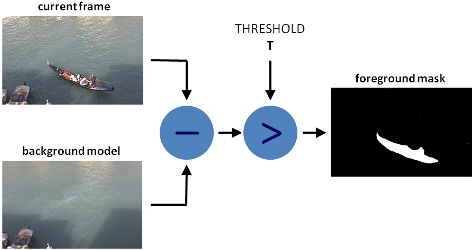
\includegraphics[width=0.618\textwidth]{images/Background_Subtraction_Tutorial_Scheme.png}
    \caption{背景减技术示意}
\end{figure}

\subsection{利用OpenCV实现背景减}

OpenCV提供了类cv::BackgroundSubstractor作背景减。在本次实验中,我们小组尝试了MOGS和KNN两种实现方法,并作对比